\section{Conclusion et perspectives}
  \begin{frame}{Conclusion et perspectives}
    \framesubtitle{}

    \begin{itemize}
      \item{La difficulté de l'extraction de termes-clés est liée à la
            discipline~:}
      \begin{figure}
        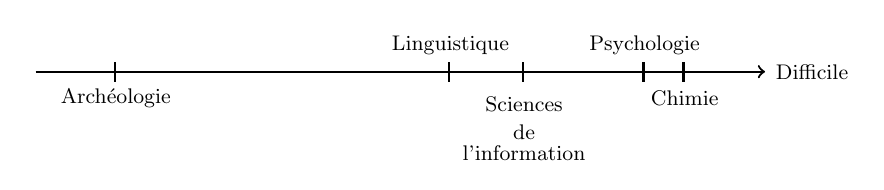
\begin{tikzpicture}[thin,
                            align=center,
                            scale=.85,
                            every node/.style={text centered, transform shape}]
          \coordinate (end) at (-4.5, 0);
          \coordinate (c) at (-5.7, 0);
          \coordinate (p) at (-6.3, 0);
          \coordinate (s) at (-8.1, 0);
          \coordinate (l) at (-9.2, 0);
          \coordinate (a) at (-14.2, 0);
          \coordinate (start) at (-15.4, 0);
          \node (chimie) at (-5.7, -0.4) {\small Chimie};
          \node (psychologie) at (-6.3, 0.4) {\small Psychologie};
          \node (sciences_de_l_information) at (-8.1, -.8) {\small Sciences\\\vspace{-.3em}\small de\\\vspace{-.3em}\small l'information};
          \node (linguistique) at (-9.2, 0.4) {\small Linguistique};
          \node (archeologie) at (-14.2, -0.4) {\small Archéologie};
          \draw[-|, thick] (start) node (facile) {} -- (a);
          \draw[-|, thick] (a) -- (l);
          \draw[-|, thick] (l) -- (s);
          \draw[-|, thick] (s) -- (p);
          \draw[-|, thick] (p) -- (c);
          \draw[->, thick] (c) -- (end) node[xshift=2em] (difficile) {\small Difficile};
        \end{tikzpicture}
      \end{figure}
      \item<2->{Deux facteurs observés~:}
      \begin{itemize}
        \item{Vocabulaire de la discipline}
        \item{Organisation du discours}
      \end{itemize}
    \end{itemize}

    \begin{block}<3->{Perspectives}
      \begin{itemize}
        \item{Mesurer automatique la difficulté a priori}
        \item{Adapter automatiquement une méthode selon la difficulté}
      \end{itemize}
    \end{block}
  \end{frame}

